\documentclass[aspectratio=169]{beamer}

% % Configurações de tema e idioma
% \usetheme{Madrid}
% \usecolortheme{default}
% \usepackage[utf8]{inputenc}
% \usepackage[T1]{fontenc}
% \usepackage[portuguese]{babel}
\usepackage{tikz}


\usetheme{PaloAlto}
\definecolor{corDoIFF}{RGB}{46,139,87}
\definecolor{Vermelho}{RGB}{255,0,0}
\definecolor{Branco}{RGB}{255,255,255}
\usecolortheme[named=corDoIFF]{structure}
\setbeamercolor{section in sidebar}{fg=Vermelho}
\setbeamercolor{section in sidebar shaded}{fg=Branco}
\addtobeamertemplate{navigation symbols}{}{%
    \usebeamerfont{footline}%
    \usebeamercolor[fg]{footline}%
    \hspace{1em}%
    \insertframenumber/\inserttotalframenumber
}

\usepackage[utf8]{inputenc}
\usepackage[portuges,brazilian]{babel}
\usepackage{listingsutf8}
\usepackage{hyperref}
\usepackage{verbatim}



% % Informações da Palestra
% \title[Ética, Integridade e IA na Pesquisa]{Ética e Integridade na Pesquisa \\ com uso da IA Generativa}
% \subtitle{Construindo a Ciência com Responsabilidade (Portaria CNPq Nº 2.664/2026)}
% \author{Palestrante Convidado}
% \institute{Comunidade Científica}
% \date{\today}


\AtBeginSection[]{
  \begin{frame}
  \vfill
  \centering
  \begin{beamercolorbox}[sep=8pt,center,shadow=true,rounded=true]{title}
    \usebeamerfont{title}\insertsectionhead\par%
  \end{beamercolorbox}
  \vfill
  \end{frame}
}

\title{Panorama de IA para Pesquisa}
%\subtitle{Panorama para docentes e discentes}
\author[Fernando Carvalho]{Fernando Carvalho}
\institute[IFF]{Instituto Federal Fluminense}
\date{}
\logo{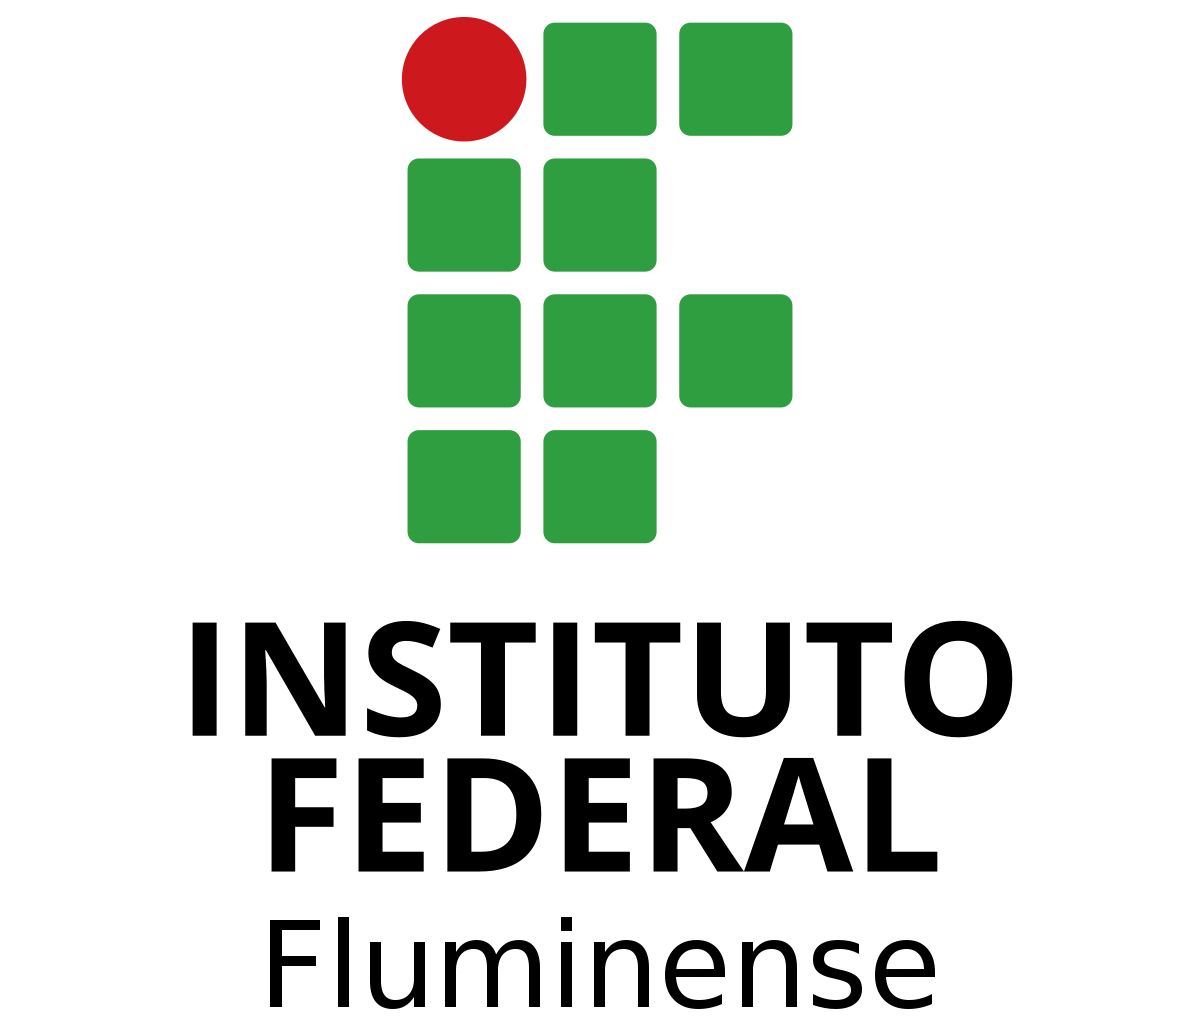
\includegraphics[scale=0.03]{logoIFF.png}}




\begin{document}

% Slide 1: Título
\begin{frame}
    \titlepage
\end{frame}


\section{Ciência: Guarda e Liderança}

% Adicione o parâmetro [t] aqui para alinhar ao topo
\begin{frame}[t]{O Propósito Maior de Fazer Ciência}

    \footnotesize
    A Ciência como Base Estrutural \\
    Fazer ciência é construir "tijolos sólidos"\space que servem de alicerce para o desenvolvimento de toda a sociedade.

    \vspace{0.3cm}
    \begin{itemize}
        \item Historicamente, a ciência focava na geração de tecnologia.
        \item A partir do Iluminismo: \textbf{a evolução da sociedade e a diminuição do sofrimento humano}.
        \item Engenheiros e Médicos precisam de conhecimento sólido e íntegro (científico).
    \end{itemize}

    % Fundo com transparência ajustado: 20% menor, alinhado à direita e ao fundo
    \begin{tikzpicture}[remember picture, overlay]
        \node[opacity=0.25, inner sep=0pt, anchor=south east] at (current page.south east) {
            \includegraphics[width=0.8\paperwidth, keepaspectratio]{tijolos da ciência 5.png}
        };
    \end{tikzpicture}

\end{frame}

\begin{frame}{Preocupações para Pesquisa}
  \centering
  \begin{itemize}
	  \item Human in the loop = Homem protagonista no circuito (processo)
	  \item IA generativa não pode ser considerada como Autor
	  \begin{itemize}
	  	\item A criação de textos deve ter o protagonismo humano
	  \end{itemize}
	  \item Autoria e escrita fazem parte da formação do pesquisador
	  \item Transparência sobre o uso da IA generativa
	  \item Uso eticamente orientado
	  \item Plágio, Originalidade e Direitos Autorais
    \item Escrita da IAG naturalmente não reconhece autores
    \begin{itemize}
        \item Não enviar dados sensíveis para IA generativa
        \item Uso de LLMs Locais como solução
    \end{itemize}
    \item Dados fabricados ou distorcidos pela IAG (Bias)
  \end{itemize}
\end{frame}

\section{Portaria}

% Slide 3: Estrutura da Portaria
\begin{frame}{A Política de Integridade do CNPq (Portaria 2.664/2026)}
    \footnotesize
    Prevenção e apuração de más condutas.
    
    \vspace{0.2cm}
    \begin{itemize}
        \item \textbf{I - Disposições Gerais:} Conceitos: má conduta como: plágio, falsificação e fabricação de dados.
        \item \textbf{\alert{II - Boas Práticas:}} Honestidade intelectual, rigor e responsabilidades.
        \item \textbf{\alert{III - Integridade:}} \textbf{regulamenta limitações e obrigações no uso de IA Generativa (IAG)}.
        \item \textbf{IV} - Comissão de Integridade (CIAC).
        \item \textbf{V} - Denúncias.
        \item \textbf{VI} - Instituições Científicas, Tecnológicas e de Inovação.
        \item \textbf{VII} - Infrações e Sanções.
        \item \textbf{VIII} - Disposições Finais: resolução de casos omissos.
    \end{itemize}
    % Palavras-chave Google Images: Documento oficial regras, balança da justiça ciência, estrutura pilares.
    % Prompt Nano Banana: A clean, stylized vector illustration of an ancient Greek pillar transforming into digital data streams at the top, representing solid rules and modern technology, minimalist, blue and white color palette, no text.
    
    % Fundo com transparência ajustado: 20% menor, alinhado à direita e ao fundo
    % \begin{tikzpicture}[remember picture, overlay]
    %     \node[opacity=0.45, inner sep=0pt, anchor=south east] at (current page.south east) {
    %         \includegraphics[width=0.6\paperwidth, keepaspectratio]{ciência e normas 3.png}
    %     };
    % \end{tikzpicture}
\end{frame}

% % Slide 5: Detalhamento Cap II
% \begin{frame}[t]{Capítulo II: Código de Boas Práticas Científicas}
%     Integridade Científica
%     \footnotesize
%     \begin{itemize}
%         \item \textbf{Princípios (Art. 6º):} Honestidade intelectual, veracidade na autoria, decoro, e respeito à justiça social, racial e de gênero.
%         \item \textbf{Deveres na Avaliação (Art. 7º):} Pareceristas devem atuar com imparcialidade, resguardar o sigilo absoluto dos dados e projetos, prevenir preconceitos e afastar-se diante de conflitos de interesses (como vínculos de parentesco ou acadêmicos).
%         \item \textbf{Transparência do Pesquisador (Art. 8º):} É obrigatório manter dados estritamente verídicos no Currículo Lattes e respeitar as regras de fomento do CNPq.
%     \end{itemize}
    
%     % Palavras-chave Google Images: Honra integridade científica, respeito diversidade, bússola ética pesquisa.
%     % Prompt Nano Banana: A modern, minimalist golden compass pointing towards a bright glowing star, resting on a clean white table, symbolizing ethical direction and moral integrity, soft natural lighting, no text.
    
% \end{frame}

% Slide 5: Detalhamento Cap II
\begin{frame}[t]{Capítulo II: Código de Boas Práticas Científicas}
    % Palavras-chave Google Images: Honra integridade científica, respeito diversidade, bússola ética pesquisa.
    % Prompt Nano Banana: A modern, minimalist golden compass pointing towards a bright glowing star, resting on a clean white table, symbolizing ethical direction and moral integrity, soft natural lighting, no text.
    \begin{itemize}
        \item \textbf{Princípios (Art. 6º):}
        \begin{itemize}
            \item Honestidade intelectual; integridade; responsabilidade;
            \item Veracidade na autoria; respeito aos participantes e objetos de pesquisa;
            \item Decoro; urbanidade; segurança; zelo pelo patrimônio;
            \item Justiça social, racial, cognitiva e de gênero;
            \item Respeito à diversidade; promoção da inclusão na ciência.
        \end{itemize}
        
        \vspace{0.4cm}
        
        \item \textbf{Deveres e Transparência do Pesquisador (Art. 8º):}
        \begin{itemize}
            \item Currículo Lattes: dados estritamente verídicos e atualizados;
            \item Normativas do CNPq: respeito às regras de bolsas e auxílios;
            \item Transparência: comunicação de afastamentos e intercorrências;
            \item Pesquisa: relato de dificuldades na execução e nos relatórios.
        \end{itemize}
    \end{itemize}
\end{frame}


% % Slide 6: Detalhamento Cap III
% \begin{frame}{Capítulo III: Diretrizes de Integridade}
%     \footnotesize
%     Estabelece o padrão rigoroso para a execução e publicação dos resultados:
    
%     \vspace{0.3cm}
%     \begin{itemize}
%         \item \textbf{Gestão e Transparência:} Exige a conservação adequada e transparente de dados, metadados e códigos em repositórios confiáveis.
%         \item \textbf{Publicação e Autoria:}
%         \begin{itemize}
%             \item Previne a chamada \textit{"Salami Science"} (fragmentação injustificada de estudos para inflar o currículo).
%             \item Exige citação fidedigna e rigorosa, diferenciando fontes primárias de secundárias e evitando o autoplágio.
%             \item Veda a "autoria fantasma" ou sem contribuição efetiva; o primeiro autor e o autor correspondente têm responsabilidade integral pela pesquisa.
%         \end{itemize}
%     \end{itemize}
%     % Palavras-chave Google Images: Repositório de dados seguro, autoria colaborativa, engrenagens publicações científicas.
%     % Prompt Nano Banana: An abstract, clean 3D illustration of transparent, interconnected glass folders glowing with data, symbolizing safe and transparent data management, minimalist white and teal colors, no text.
% \end{frame}

% Slide 6: Detalhamento Cap III
\begin{frame}[t]{Capítulo III: Diretrizes de Integridade}
    % Palavras-chave Google Images: Repositório de dados seguro, autoria colaborativa, engrenagens publicações científicas.
    % Prompt Nano Banana: An abstract, clean 3D illustration of transparent, interconnected glass folders glowing with data, symbolizing safe and transparent data management, minimalist white and teal colors, no text.
    \footnotesize
    Padrão rigoroso para a execução e publicação de resultados:
    
    \vspace{0.3cm}
    \begin{itemize}
        \item \textbf{Gestão e Transparência:}
        \begin{itemize}
            \item Conservação adequada; dados, metadados, protocolos, códigos e software;
            \item Transparência e integridade; depósito em repositórios confiáveis.
        \end{itemize}
        
        \vspace{0.2cm}
        
        \item \textbf{Publicação e Autoria:}
        \begin{itemize}
            \item Citação rigorosa e fidedigna; distinção clara entre fontes primárias e secundárias;
            \item Prevenção ao autoplágio;
            \item Combate à \textit{"Salami Science"} (fragmentação injustificada de resultados);
            \item Autoria legítima: exigência de contribuição efetiva;
            \item Vedada "autoria fantasma"; proibição de compra/venda de autoria;
            \item Responsabilidade integral (foco no primeiro autor e autor correspondente);
            \item Repúdio a periódicos, eventos ou editais predatórios.
        \end{itemize}
    \end{itemize}
\end{frame}

\section{Casos Práticos}

% Slide 4: Tópicos sobre IA Generativa
\begin{frame}[t]{Uso da IA Generativa (IAG) nas Diretrizes do CNPq}
    \footnotesize
    A Portaria aponta deveres no uso de ferramentas de IA:
    
    \vspace{0.2cm}
    \begin{enumerate}
        \item \textbf{Declaração de Uso:} obrigatório declarar: qual, quando, onde, de que forma, qual finalidade.
        \item \textbf{Vedação de Falsa Autoria:} É proibido conteúdo gerado por IA como se fosse de autoria humana.
        \item \textbf{Responsabilidade Integral:} O autor responde integralmente pelo conteúdo (plágios, imprecisões).
        \item \textbf{Proteção ao Sigilo:} É \textbf{vedada} projetos não públicos em IAG (pareceres, ...).
    \end{enumerate}
    % Palavras-chave Google Images: IA lupa transparência, colaboração humano robô, cadeado sigilo pesquisa.
    % Prompt Nano Banana: A simple graphic of a glowing magnifying glass hovering over a futuristic digital document, symbolizing transparency and analysis in AI, dark background with cyan neon accents, highly polished, no text.
    
    % Fundo com transparência ajustado: 20% menor, alinhado à direita e ao fundo
    \begin{tikzpicture}[remember picture, overlay]
        \node[opacity=0.45, inner sep=0pt, anchor=south east] at (current page.south east) {
            \includegraphics[width=0.6\paperwidth, keepaspectratio]{proibicao_protecao_sigilo 1.png}
        };
    \end{tikzpicture}

\end{frame}

% Slide 7: Tabela de Casos Práticos (Inserir antes do detalhamento dos Capítulos)
\begin{frame}{Casos Práticos com IA Generativa: O que pode e o que não deve?}
    \scriptsize % Fonte reduzida para acomodar a tabela sem poluir o slide
    \begin{center}
        \renewcommand{\arraystretch}{1.2} % Aumenta o espaçamento entre as linhas
        \vspace{-1}
        \begin{tabular}[t]{|p{4.5cm}|c|p{6.5cm}|}
            \hline
            \textbf{Situação (Ação com a IA)} & \textbf{Veredito} & \textbf{Porquê?} \\
            \hline
            IA gerar a problematização & \textcolor{red}{\textbf{NÃO deve}} & IA não deveria construir o raciocínio e o argumento no lugar do \textbf{Humano}. \\
            \hline
            \textbf{Humano} criar insights, fichamentos e ideias e pedir estruturação & \textcolor{blue}{\textbf{PODE}} & Conteúdo original \textbf{Humano}; IA como ferramenta, só o organiza tecnicamente. \\
            \hline
            IA ler artigos e gerar o referencial teórico & \textcolor{red}{\textbf{NÃO deve}} & Terceiriza a leitura, compreensão, análise, seleção e a construção do argumento teórico. \\
            \hline
            Usar fichamentos/citações dos artigos feitos por IA  & \textcolor{red}{\textbf{NÃO deve}} & O fichamento faz parte da interpretação; exige leitura e reflexão, não é só tarefa mecânica. \\
            \hline
            IA para estudar, entender, analisar artigos \textbf{já lidos} & \textcolor{blue}{\textbf{PODE}} & Leitura, análise, racional \textbf{Humana}; IA apenas apoia a compreensão. \\
            \hline
            Publicar a análise e o racional da IA sobre dados coletados & \textcolor{red}{\textbf{NÃO deve}} & A análise exige interpretação autoral; um \textbf{Humano} precisa ser o responsável pelos achados. \\
            \hline
            IA para melhorar a estrutura e apresentação da análise \textbf{Humana} & \textcolor{blue}{\textbf{PODE}} & Interpretação \textbf{Humana}; IA melhora a apresentação. \\
            \hline
            IA para revisar gramática, clareza e fluidez & \textcolor{blue}{\textbf{PODE}} & IA não foi responsável pelo conteúdo intelectual. \\
            \hline
        \end{tabular}
    \end{center}
\end{frame}


\section{Reflexões}

% Slide 8: Conclusão
\begin{frame}[t]{Reflexões para casa ...}
    \footnotesize
    \begin{itemize}
        \item Adaptação para uso da IAG é inevitável, e pode produzir bons resultados.
        \item Podemos usar IAG com ética para promover o desenvolvimento científico.
        \item Tem que haver protagonismo Humano e curadoria do que passe pela IA.
    \end{itemize}
        \vspace{1}
    \begin{itemize}
        \item Fazer ciência é uma responsabilidade social. Os "tijolos"\space que construímos hoje devem ser moldados pela \textbf{honestidade intelectual} (Cap. II) e pelas \textbf{diretrizes rigorosas de publicação e gestão de dados} (Cap. III).
        \item A Inteligência Artificial é uma ferramenta poderosa, mas exige total transparência e \textbf{não deve substitui a autoria, a análise, as decisões, nem a responsabilidade humana}.
        \item Por fim, a ciência precisa ser norteada pela \textbf{ética e integridade científica}, visando sempre a construção de uma sociedade evoluída, que \textbf{não aceita o sofrimento humano}.
    \end{itemize}
    % Palavras-chave Google Images: Mundo melhor ciência, humanidade prosperando, nascer do sol esperança inovação.
    % Prompt Nano Banana: A serene, beautiful sunrise over a clean, futuristic but nature-filled city, symbolizing a highly evolved society free of suffering built on ethical science, minimalistic art style, hopeful and inspiring mood, no text.

\end{frame}

\section{Referências}

% Slide 8: Referências Bibliográficas
\begin{frame}{Referências Bibliográficas}
    \footnotesize 
    \begin{itemize}
        \item \textbf{Normativas e Guias Oficiais:}
        \begin{itemize}
            \item BRASIL. Conselho Nacional de Desenvolvimento Científico e Tecnológico (CNPq). \textit{Portaria CNPq Nº 2.664, de 6 de março de 2026. Institui a Política de Integridade na Atividade Científica do CNPq}. Publicado no DOU de 11 de março de 2026.
            
            \vspace{0.2cm}
            
            \item BRASIL. Secretaria de Governo Digital (SGD). \textit{Cartilha IA Generativa}. Governo Digital. Disponível em: \\ \url{https://www.gov.br/governodigital/pt-br/infraestrutura-nacional-de-dados/inteligencia-artificial-1/publicacoes/cartilha-ia-generativa}
        \end{itemize}
        
        \vspace{0.4cm}
        
        \item \textbf{Material Complementar Recomendado:}
        \begin{itemize}
            \item Vídeo de apoio e discussão sobre o tema: \href{https://www.youtube.com/watch?v=6yiHXPxoI6Q}{IA na pesquisa | Portaria CNPq 2026}
        \end{itemize}
    \end{itemize}
\end{frame}

\begin{frame}{Referências Bibliográficas}

    \vspace{0.6cm}
    \begin{center}
        \textbf{Obrigado!}
    \end{center}
\end{frame}



\end{document}

